\ifslide{

  \section{Agenda}
  \begin{frame}{Agenda}
    \begin{block}{Session outline}
      \begin{itemize}
        \item functions
        \item data conversion
        \item data structure (classe)
        \item error handling
        \item objects and methods
      \end{itemize}
    \end{block}
  \end{frame}
}


\ifslide{

    \begin{frame}{No session on the 15.06}
      \begin{block}{No class on the 15.06}
        \begin{itemize}
          \item postpone to 22.06 ?
          \item postpone to 06.07 ?
        \end{itemize}
      \end{block}
    \end{frame}

}

\section{Functions}

\ifslide{
  \begin{frame}
    \begin{block}{What is function ?}
       \textit{In computer science, a subroutine, also termed procedure, function, routine, method, or
       subprogram, is a part of source code within a larger computer program that performs a specific
       task and is relatively independent of the remaining code. - Wikipedia
       \mylink{http://en.wikipedia.org/wiki/Subroutine}{"Subroutine"}, accessed
       the 22.05.2012}
    \end{block}

    \begin{block}{What are their purpose ?}
      \begin{itemize}
        \item reuse code easily
        \item make code easier to read
        \item breakdown code in different, meaningful, part
        \item hide complexity
      \end{itemize}
    \end{block}
  \end{frame}

  \begin{frame}
    \begin{block}{Functions syntax}
      \begin{center}
        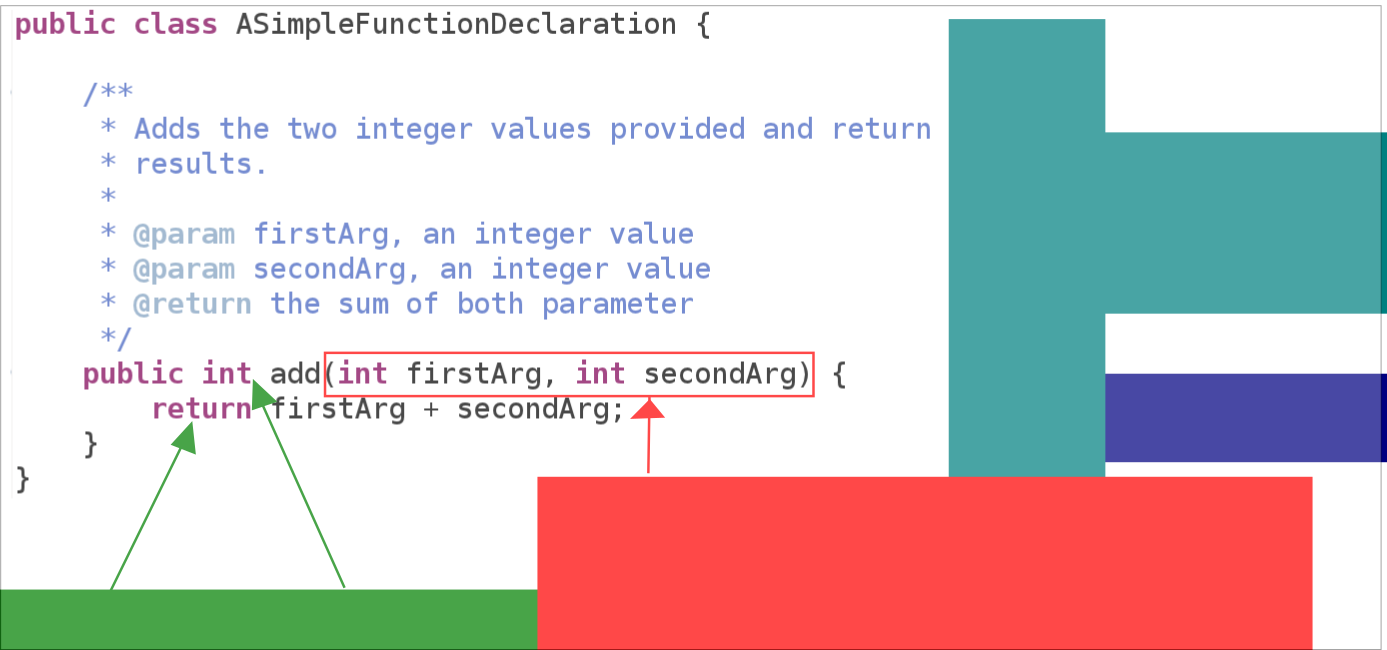
\includegraphics[scale=0.3]{../img/a-simple-java-function.png}
      \end{center}
    \end{block}
  \end{frame}

  \begin{frame}
    \begin{block}{Exercice 1: Create a simple function to add two integer}
      \begin{itemize}
        \item Create a Java file in your project called FunctionByExample with a right-click on the
        folder containing the Java source files
        \item \textit{Remark: Check the option "public static void main..." in the form
        \item Add to the class the following function:
        \begin{itemize}
          \item \texttt{public static int add(int a, int b)}
          \item implements the body of the function
        \end{itemize}
        \item Remark: the function must be \textbf{within} the class definition
        \item in the \textbf{main} function add a call to the add function:
        \begin{itemize}
          \item \texttt{FunctionByExample.add(1,2)}
        \end{itemize}
      \end{itemize}
    \end{block}
  \end{frame}


  \begin{frame}
    \begin{block}{Exercice 1: Reduce code duplication in using functions}
      \begin{itemize}
        \item Import your Eclipse project the file called LenghtyProgram
        \item Follow the instructions and modify the code accordingly
      \end{itemize}
    \end{block}
  \end{frame}
}

\section{Data Conversion}
\ifslide{
  \begin{frame}
    \begin{block}{Data conversion}
      \begin{itemize}
        \item variables holds \textbf{typed} data
        \item need to convert one to an other:
        \begin{itemize}
          \item an integer (3) to a float (3.0)
          \item a char (c) to the
          \item a String ("1.0") to a float (1.0)
        \end{itemize}
        \item in Java, this can be achieved by some provided functions:
        \begin{itemize}
          \item \texttt{int value = Integer.valueOf("1.0");}
          \item \texttt{short value = Short.valueOf(1.0f);}
          \item \texttt{float value = Float.valueOf(1);}
        \end{itemize}
      \end{itemize}
    \end{block}
  \end{frame}
}
\section{Constants}
\ifslide{
  \begin{frame}
    \begin{block}{Constants}
      \begin{itemize}
        \item some variable never changes
        \item can be prefixed by keyword \texttt{final}
        \item to prevent any - unwanted, changes later in the program
        \item convention is, in most languages, to use uppercase variable:
        \begin{itemize}
          \item \texttt{final long EARTH\_DIAMETER = 12,714;}
          \item \texttt{final float PIE = 3. 1415926535;}
        \end{itemize}
      \end{itemize}
    \end{block}
  \end{frame}
}

\ifslide{

  \begin{frame}
    \begin{block}{Exercice 2: Increase code structuration using functions}
      \begin{itemize}
        \item Import your Eclipse project the file called TiedlyCoupledBusinessCode
        \item Follow the instructions and modify the code accordingly
      \end{itemize}
    \end{block}
  \end{frame}
}

\section{Data Structure}
\ifslide{
  \begin{frame}
    \begin{block}{What to modelize complex data ?}
      \begin{itemize}
        \item concept of \textbf{data structure}
        \item define a new \textbf{type} of variable
        \item that regroups all variables
        \item in Java, a data structure is called \textbf{class}
      \end{itemize}
    \end{block}
    \begin{center}
      \includegraphics[scale=0.4]{img/datastructure.png}
    \end{center}
  \end{frame}

  \begin{frame}
    \begin{block}{How to use a data structure ?}
      \begin{itemize}
        \item inner variables can be accessed directly
        \begin{itemize}
          \item \texttt{steuerzahler.id = 120304;}
        \end{itemize}
        \item structure can be passed around di
        \begin{itemize}
          \item \texttt{public static void calculateTax(Steuerzahler steuerzahler) ...}
        \end{itemize}
      \end{itemize}
    \end{block}
  \end{frame}

  \begin{frame}
    \begin{block}{Designing a data structure}
      \begin{itemize}
        \item Create a new \textbf{class}:
        \begin{itemize}
          \item Right click on the folder containing your source code (inside Eclipse)
          \item Select New...->Java Class
          \item Name the new class Consultant
        \end{itemize}
        \item a Consultant's data structure should regroup the following information:
        \begin{itemize}
          \item an unique id value
          \item years of experience
          \item a country code (where he works) identified by two letter (DE, UK, FR...)
          \item cost by day ratio (how much the consultant is sold by day)
          \item a phone number
        \end{itemize}
        \item implements the data structure
        \item add the following function to the class and implement it:
        \begin{itemize}
          \item \texttt{public static int consultantCostFor(Consultant consultant, int nbDays);}
        \end{itemize}
      \end{itemize}
    \end{block}
  \end{frame}
}


\section{Error Handling}
\ifslide{
 \begin{frame}
    \begin{block}{Structure to handle error in programming language}
      \begin{itemize}
        \item do nothing
        \begin{itemize}
          \item program crashes
          \item no information on the root cause
        \end{itemize}
        \item use "status code"
        \begin{itemize}
          \item functions can't return value
          \item leads to message such as "Error 400 happened"
          \item needs to have an error database to translate the status code
        \end{itemize}
        \item return a complete structure describing in length the error
        \begin{itemize}
          \item ideal, but...
          \item ...still remove the option of having returning value
        \end{itemize}
        \item hence appeared the idea of \textbf{exception}
        \begin{itemize}
          \item returns a complete structure describing the error
          \item does not modify the return type of a function
          \item can be explicitly catched or not
          \item can be explicitly thrown or not
        \end{itemize}
      \end{itemize}
    \end{block}
 \end{frame}

 \begin{frame}
   \begin{center}
     \includegraphics[scale=0.30]{img/exception-in-java.png}
   \end{center}
 \end{frame}
}



